%----------------------------------------------------------------------------------------
% Cadenas de Márkov
%----------------------------------------------------------------------------------------

En esta práctica se implementarán funciones para realizar cálculos básicos sobre cadenas de Márkov.

\section{Objetivo}

\begin{compactitem}
 \item Que el alumno se familiarice con los procesos estocásticos discretos denominados Cadenas de Márkov discretas y realice una implementación para resolver algunas de las preguntas más frecuentes que se pueden plantear sobre estos procesos.
\end{compactitem}


\section{Introducción}

\begin{figure}
 \centering
 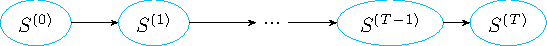
\includegraphics[width=0.8\textwidth]{markov/CadenaDeMarkov}
 \caption{Una Cadena de Márkov es una Red de Bayes degenerada.}\label{Fig:CadenaDeMarkov}
\end{figure}

\begin{definition}[Cadena de Márkov discreta]
 \begin{itemize}
  \item Una \emph{Cadena de Márkov} es un modelo bayesiano dinámico donde cada nodo representa el estado del sistema al tiempo $t$, denotado $S^{(t)}$, y éste sólo tiene un padre: el estado del sistema en el tiempo anterior $S^{t-1}$. [\fref{Fig:CadenaDeMarkov}]

  \item El sistema tiene un conjunto finito de estados discretos posibles $S = \{s_1,...,s_n\}$

  \item Asume \emph{invarianza temporal}, es decir, la probabilidad de transición $P(S^{(t+1)}|S^{(t)})$ es la misma para todo $t$.
 \end{itemize}
\end{definition}

\subsection{Inferencia}

Frecuentemente la probabilidad de transición de un estado a otro se expresa con un autómata al plantear el problema.  De este autómata es posible extraer el factor representando la probabilidad condicionar $P(S^{(t+1)}|S^{(t)})$, con las variables $S^{(t)}$ y  $S^{(t+1)}$ en su alcance.

Si a esto agregamos el factor con la distribución de probabilidad para el estado inicial $P(S^{(0)})$, es posible obtener $P(S^{(t)})$ para cualquier $t$ utilizando la regla de la cadena de Bayes.  Por ejemplo, para $t=1$:
\begin{align*}
 P(S^{(1)}) = \sum_{S^{(0)}} P(S^{(1)}|S^{(0)}) P(S^{(0)})
\end{align*}
con lo que obtenemos la probabilidad del que el sistema se encuentre en cualquier estado al tiempo $t=1$, independientemente de en qué estado haya iniciado.

Recursivamente:
\begin{align*}
 P(S^{(t+1)}) = \sum_{S^{(t)}} P(S^{(t+1)}|S^{(t)}) P(S^{(t)})
\end{align*}

Sin embargo, utilizar factores puede ser un cañón para este caso, pues cada nodo sólo tiene un nodo padre.  Podemos notar que la multiplicación de factores y marginalización sobre la variable padre, se pueden realizar en una sola operación si escribimos la distribución de probabilidad condicional en una matriz:
\begin{align*}
 T &= \begin{bmatrix}
        P(S=s_1|S=s_1) & ... & P(S=s_1|S=s_n) \\
        P(S=s_2|S=s_1) & ... & P(S=s_2|S=s_n) \\
        ... \\
        P(S=s_n|S=s_1) & ... & P(S=s_n|S=s_n) \\
       \end{bmatrix} \\
\end{align*}
y la distribución de probabilidad para el estado en cada tiempo con un vector:
\begin{align*}
  P(S) &= \begin{bmatrix}
	  P(s_1) \\
	  P(s_2) \\
	  ...\\
	  P(s_n)
	 \end{bmatrix}
\end{align*}
Entonces el cálculo de la distribución de probabilidad para otros tiempos se resume como:
\begin{align*}
 P(S^{t+1}) &= T P(S^{t}) \\
 P(S^{t+1}) &= T^n P(S^{0})
\end{align*}


\subsection{Ejemplo: El soldado}

Supongamos que estamos modelando el comportamiento de un soldado en un videojuego de acción.  Este soldado está vigilando un área restringida y puede tener alguno de tres comportamientos: estar caminando, quedarse de pie o dormido.  El estado del soldado queda descrito por la variable $S \in \{caminando, dormido, de\ pie\}$, lo cual en ocasiones abreviaremos como $S \in \{cam, dor, d.p.\}$.  Para que su comportamiento no sea tan predecible, cambiará su actividad aleatoriamente según describe el autómata en la \fref{Fig:SoldadoMarkov}.

\begin{figure}
 \centering
 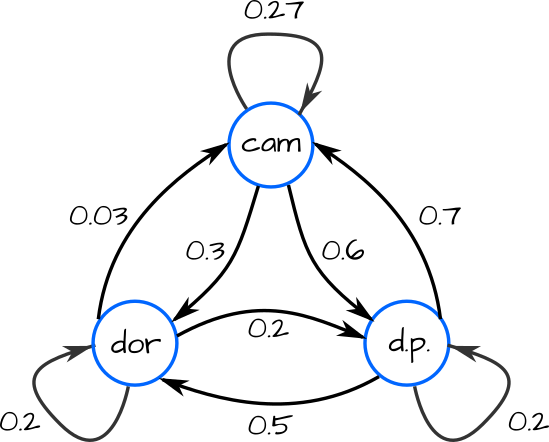
\includegraphics[width=0.4\textwidth]{markov/SoldadoMarkov}
 \caption{Las probabilidades de transición expresadas con un autómata.}\label{Fig:SoldadoMarkov}
\end{figure}

Entonces, la matriz de transición se acomoda como en la tabla siguiente:

 \begin{center}
 \begin{tabular}{l|ccc}
  \multicolumn{4}{c}{$P(S^{(t+1)}|S^{(t)})$} \\ \hline
  $S^{(t+1)}$ \textbackslash $S^{(t)}$          & caminando & dormido & de pie \\ \hline
  caminando &    0.27   &    0.3  & 0.6 \\
  dormido   &    0.03   &    0.2  & 0.2 \\
  de pie    &    0.7    &    0.5  & 0.2
 \end{tabular}
 \end{center}

 Inicialmente sea:

 \begin{center}
 \begin{tabular}{l|c}
  \multicolumn{1}{c|}{$S^{(0)}$}   &  $P(S^{(0)})$ \\ \hline
  caminando &    0.2 \\
  dormido   &    0.2 \\
  de pie    &    0.6
 \end{tabular}
 \end{center}



Adicionalmente a lo visto en clase, que estuvo basado en el sitio de \hrefformat{https://www.gestiondeoperaciones.net/cadenas-de-markov/cadenas-de-markov-ejercicios-resueltos/}{Gestión de operaciones}, pueden consultar la página sobre cadenas de Márkov en \hrefformat{https://en.wikipedia.org/wiki/Markov_chain}{Wikipedia} así como algunos \hrefformat{https://en.wikipedia.org/wiki/Examples_of_Markov_chains}{ejemplos} sencillos.


\section{Desarrollo}

Para esta práctica se requiere implementar una clase para trabajar con cadenas de Márkov.  Se recomienda programarla en \code{Python}, ya que la biblioteca \code{numpy} contiene métodos para trabajar con matrices y vectores, lo cual simplifica mucho los puntos siguientes.  También se recomienda utilizar matrices columna para representar vectores, de esta manera funcionarán correctamente las multiplicaciones de matriz por vector.

La clase \code{CadenaDeMarkov} debe contener:

\begin{enumerate}
 \item Un constructor que reciba como parámetros:
 \begin{enumerate}
  \item Una lista con los nombres los estados posibles.
  \item Un vector con la probabilidad de iniciar en cada uno de los estados posibles.
  \item Una matriz de probabilidades, con la probabilidad de transitar de cada estado hacia los demás.
 \end{enumerate}

 \item Un método para generar una secuencia de estados a partir del modelo de Márkov iniciado dado el número $n$ de elementos que tendrá la secuencia; opcionalmente puede recibir como parámetro una semilla para la generación de números aleatorios.
 
 Para generar esta muestra necesitarás calcular los vectores con las distribuciones de probabilidad para $n$ pasos.  Dada cada distribución, utiliza un número aleatorio para determinar cuál de los estados corresponderá a ese paso.
 
 Devuelve una lista con la secuencia de estados.
 
 \item Obtener la probabilidad de una cadena de estados (punto extra si se permite que esta cadena tenga estados indeterminados).  Observa que esta es la distribución de probabilidad conjunta $P(S_0=s_0,S_1=s_1,...,S_n=s_n)$, escrito de otra forma, $P(s_0,s_1,...,s_n)$.  Deberá recibir como parámetro una lista con la secuencia de estados y devolver la probabilidad.
 
 \item Estimar las probabilidades a largo plazo de cada uno de los estados, es decir, la distribución límite, cuando sea posible.  Este método deberá devolver el vector con la distribución de probabilidades.
 
 \item Agregar un archivo donde se utilice tu clase para resolver un ejemplo, usando cada uno de los métodos.  Puedes usar algún ejemplo del sitio de gestión de operaciones.
\end{enumerate}


\subsection{Requisitos y resultados}

Incluir:

\begin{enumerate}
 \item El archivo de la clase \code{CadenaDeMarkov}.
 \item El archivo con el demo de prueba.
\end{enumerate}

